\documentclass[border=10pt]{standalone}
\usepackage[svgnames]{xcolor}
\usepackage{amsmath}
\usepackage{pgfplots}
\pgfplotsset{compat=newest}
\usepackage[sfdefault]{FiraSans}
\usepackage{FiraMono}
\renewcommand*\familydefault{\sfdefault}
\begin{document}
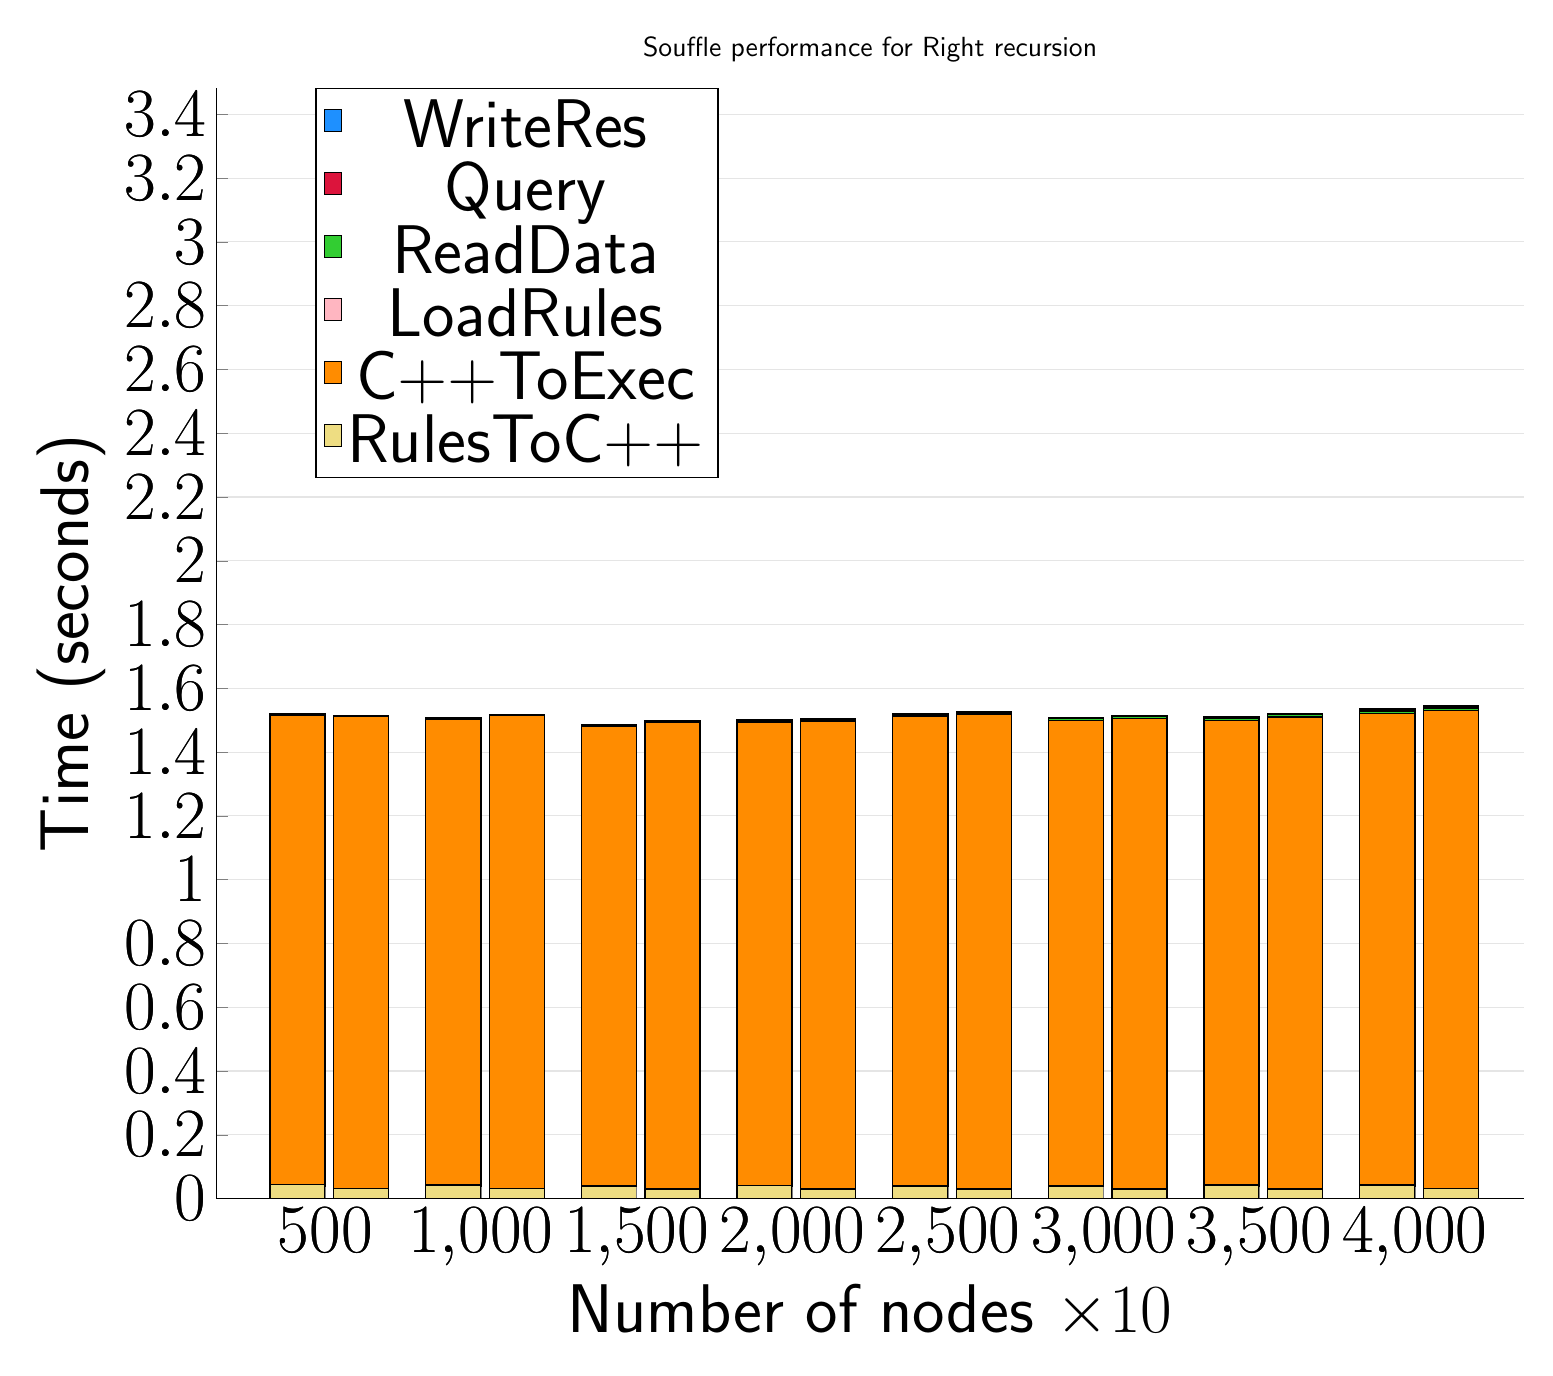
\begin{tikzpicture}
	\begin{axis}[
			ybar stacked,
			title={Souffle performance for Right recursion},
			bar shift=-10pt,
			width=1.5\textwidth,
			bar width=0.7cm,
			ymajorgrids, tick align=inside,
			major grid style={draw=gray!20},
			xtick=data,
			ymin=0, ymax=3.4829999923706056,
			axis x line*=bottom,
			axis y line*=left,
			enlarge x limits=0.1,
			legend style={
					at={(0.23, 1)},
					anchor=north,
					legend columns=1,
					font=\Huge,
				},
			ylabel={Time (seconds)},
			xlabel={Number of nodes $\times 10$},
			label style={font=\Huge},
			tick label style={font=\Huge},
		]
		\addlegendimage{fill=DodgerBlue, draw=black, line width=0.2pt}
		\addlegendentry{WriteRes}
		\addlegendimage{fill=Crimson, draw=black, line width=0.2pt}
		\addlegendentry{Query}
		\addlegendimage{fill=LimeGreen, draw=black, line width=0.2pt}
		\addlegendentry{ReadData}
		\addlegendimage{fill=LightPink, draw=black, line width=0.2pt}
		\addlegendentry{LoadRules}
		\addlegendimage{fill=DarkOrange, draw=black, line width=0.2pt}
		\addlegendentry{C++ToExec}
		\addlegendimage{fill=LightGoldenrod, draw=black, line width=0.2pt}
		\addlegendentry{RulesToC++}
		\addplot +[fill=LightGoldenrod, draw=black, line width=0.5pt] coordinates {
				(500, 0.04399995803833008)
				(1000, 0.04200003147125244)
				(1500, 0.03900001049041748)
				(2000, 0.040999960899353025)
				(2500, 0.039999985694885255)
				(3000, 0.039999985694885255)
				(3500, 0.04200000762939453)
				(4000, 0.04200000762939453)
			};
		\addplot +[fill=DarkOrange, draw=black, line width=0.5pt] coordinates {
				(500, 1.4730000495910645)
				(1000, 1.4609999895095824)
				(1500, 1.4420000076293946)
				(2000, 1.4520000219345093)
				(2500, 1.4730000019073486)
				(3000, 1.4589999914169312)
				(3500, 1.4579999923706055)
				(4000, 1.4789999961853026)
			};
		\addplot +[fill=LightPink, draw=black, line width=0.5pt] coordinates {
				(500, 1.32625e-05)
				(1000, 0.0)
				(1500, 0.0)
				(2000, 1e-05)
				(2500, 0.0)
				(3000, 0.0)
				(3500, 1.01042e-05)
				(4000, 0.0)
			};
		\addplot +[fill=LimeGreen, draw=black, line width=0.5pt] coordinates {
				(500, 0.0013731659999999999)
				(1000, 0.00241673)
				(1500, 0.003634092)
				(2000, 0.004752129)
				(2500, 0.004937317)
				(3000, 0.005823404)
				(3500, 0.0071710789999999995)
				(4000, 0.00851351)
			};
		\addplot +[fill=Crimson, draw=black, line width=0.5pt] coordinates {
				(500, 0.0005306751)
				(1000, 0.0010614040000000002)
				(1500, 0.001597776)
				(2000, 0.002071038)
				(2500, 0.002274788)
				(3000, 0.002682617)
				(3500, 0.003425487)
				(4000, 0.003971268)
			};
		\addplot +[fill=DodgerBlue, draw=black, line width=0.5pt] coordinates {
				(500, 0.0004327292)
				(1000, 0.0006342291000000001)
				(1500, 0.0008954248000000002)
				(2000, 0.0010658755000000002)
				(2500, 0.0011173267)
				(3000, 0.0012495875)
				(3500, 0.001536062)
				(4000, 0.0017749250000000001)
			};
	\end{axis}
	\begin{axis}[
			ybar stacked,
			bar shift=13pt,
			width=1.5\textwidth,
			bar width=0.7cm,
			ymajorgrids, tick align=inside,
			major grid style={draw=none},
			xtick=data,
			ymin=0, ymax=3.4829999923706056,
			axis x line*=none,
			axis y line*=none,
			enlarge x limits=0.1,
			label style={font=\Huge},
			tick label style={font=\Huge},
		]
		\addplot +[fill=LightGoldenrod, draw=black, line width=0.5pt] coordinates {
				(500, 0.031000000000000007)
				(1000, 0.031000000000000007)
				(1500, 0.030000000000000006)
				(2000, 0.030000000000000006)
				(2500, 0.030000000000000006)
				(3000, 0.030000000000000006)
				(3500, 0.030000000000000006)
				(4000, 0.031)
			};
		\addplot +[fill=DarkOrange, draw=black, line width=0.5pt] coordinates {
				(500, 1.4809999999999999)
				(1000, 1.483)
				(1500, 1.4640000000000002)
				(2000, 1.4669999999999999)
				(2500, 1.488)
				(3000, 1.475)
				(3500, 1.4800000000000002)
				(4000, 1.499)
			};
		\addplot +[fill=LightPink, draw=black, line width=0.5pt] coordinates {
				(500, 1.32e-05)
				(1000, 0.0)
				(1500, 0.0)
				(2000, 0.0)
				(2500, 0.0)
				(3000, 0.0)
				(3500, 1e-05)
				(4000, 0.0)
			};
		\addplot +[fill=LimeGreen, draw=black, line width=0.5pt] coordinates {
				(500, 0.0013585)
				(1000, 0.0023988000000000004)
				(1500, 0.0036106000000000007)
				(2000, 0.0046609)
				(2500, 0.0048955)
				(3000, 0.0057937)
				(3500, 0.007134800000000001)
				(4000, 0.008418100000000001)
			};
		\addplot +[fill=Crimson, draw=black, line width=0.5pt] coordinates {
				(500, 0.0005299)
				(1000, 0.0010607000000000001)
				(1500, 0.0015976)
				(2000, 0.0020704000000000005)
				(2500, 0.0022706)
				(3000, 0.0026808000000000005)
				(3500, 0.0033788)
				(4000, 0.0039652)
			};
		\addplot +[fill=DodgerBlue, draw=black, line width=0.5pt] coordinates {
				(500, 0.0004182)
				(1000, 0.0006336)
				(1500, 0.0008641999999999999)
				(2000, 0.0010643999999999999)
				(2500, 0.0011023)
				(3000, 0.0012483)
				(3500, 0.0015306999999999999)
				(4000, 0.0017563000000000001)
			};
	\end{axis}
\end{tikzpicture}

\end{document}
